\emph{\underline{Objetivo:}}\\

Se inicia la sesi\'on con el PDA abri\'endose as\'i la aplicaci\'on. Al iniciar la sesi\'on ser\'a necesario que el usuario introduzca su clave y nombre de usuario, que de ser correctos le dar\'an acceso a los men\'us.	\\

\emph{\underline{Entradas:}}
\begin{itemize}
\item Clave de usuario.
\item Nombre de usuario.
\end{itemize}

\emph{\underline{Precondiciones:}}\\

No hay precondiciones.\\

\emph{\underline{Salidas:}}\\
	
En caso de \'exito (clave y nombre de usuario son correctos): 
\begin{itemize}
	\item Se muestra el men\'u de la aplicaci\'on en la pantalla del PDA.
\end{itemize}

En caso de fallo (clave y nombre de usuario no son correctos): 
\begin{itemize}
	\item Se informa al usuario de que los datos introducidos no son correctos.
	\item Se vuelve a la pantalla de inicio para que el usuario tenga la posibilidad de volver  a intentar iniciar la sesi'on.
\end{itemize}

\emph{\underline{Postcondici\'on si \'exito (clave y nombre de usuario son correctos):}}\\

Se muestra el men\'u de la aplicaci\'on por la pantalla del PDA.\\

\emph{\underline{Postcondici\'on si fallo (clave y nombre de usuario no son correctos):}}\\

Se informa al usuario de que los datos introducidos no son correctos y se le ofrece la posibilidad de intentar acceder a la aplicaci\'on de nuevo.\\

\emph{\underline{Actores: }}
\begin{itemize}
	\item Usuario con PDA.
	\item Servidor del hospital.
	\item PDA.
\end{itemize}

\emph{\underline{Secuencia normal:}}
\begin{enumerate}
	\item Al encender el PDA, se solicita al usuario que introduzca su clave y su nombre de usuario y \'estos son enviados a la base de datos del servidor del hospital para que sean verificados.
	\item El servidor busca en su base de datos la clave y el nombre de usuario que se acaban de introducir para confirmar que est\'a iniciando sesi\'on una persona autorizada, personal del hospital. En caso de que la b\'usqueda tenga \'exito pasar a 3, en caso contrario pasar a E1.
	\item Una vez confirmada la clave y el nombre de usuario, en el PDA tenemos disponible el men\'u con todas las posibles operaciones que se pueden realizar con la aplicaci\'on.
\end{enumerate}

\emph{\underline{Secuencias alternativas:}}\\

E1.- Se informa al usuario de que los datos que ha introducido no son correctos y se le da la oportunidad de volver a introducirlos (paso 1).\\
\\\\

Para ilustrar mejor est'a secuencia de acciones, incluimos el diagrama de secuencia de este caso de uso:\\

\begin{figure*}[h!]
	\begin{center}
        		\framebox{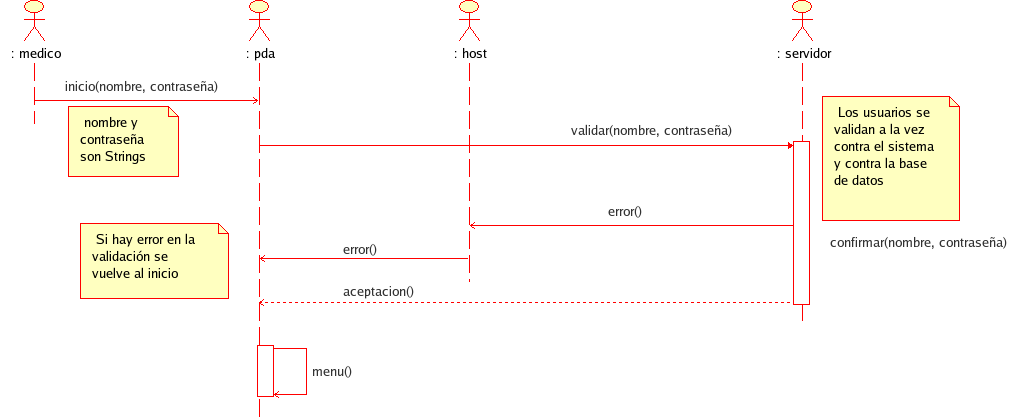
\includegraphics[width=1.0\textwidth]{dsecuenciainicio.png}}
     	\end{center}
    	\caption{Diagrama de secuencia del inicio de sesi'on}\label{fig:inicio_sesion}
\end{figure*}